%%%%%%%%%%%%%%%%%%%%%%%%%%%%%%%%%%%%%%%%%
% University/School Laboratory Report
% LaTeX Template
% Version 3.1 (25/3/14)
%
% This template has been downloaded from:
% http://www.LaTeXTemplates.com
%
% Original author:
% Linux and Unix Users Group at Virginia Tech Wiki 
% (https://vtluug.org/wiki/Example_LaTeX_chem_lab_report)
%
% License:
% CC BY-NC-SA 3.0 (http://creativecommons.org/licenses/by-nc-sa/3.0/)
%
%%%%%%%%%%%%%%%%%%%%%%%%%%%%%%%%%%%%%%%%%

%----------------------------------------------------------------------------------------
%	PACKAGES AND DOCUMENT CONFIGURATIONS
%----------------------------------------------------------------------------------------

\documentclass{article}

\usepackage{graphicx} % Required for the inclusion of images
\usepackage{amsmath} % Required for some math elements
\usepackage{enumitem}
\usepackage[section]{placeins}

\setlength\parindent{0pt} % Removes all indentation from paragraphs

\renewcommand{\labelenumi}{\alph{enumi}.} % Make numbering in the enumerate environment by letter rather than number (e.g. section 6)

\newlist{inlinelist}{enumerate*}{1}
\setlist*[inlinelist,1]{%
  label=(\arabic*),
}

%----------------------------------------------------------------------------------------
%	DOCUMENT INFORMATION
%----------------------------------------------------------------------------------------

\title{\begin{LARGE}
	\textbf{EE 445L - Lab 7: Design and Layout of an Embedded System}
\end{LARGE}} % Title

\author{Joshua Bryant \\ jmb6357 \and James Morris \\ jsm3288} % Author name

\date{\today} % Date for the report

\begin{document}

\maketitle % Insert the title, author and date

%----------------------------------------------------------------------------------------
%	SECTION 1 Objectives
%----------------------------------------------------------------------------------------

\section{Objectives}

		\subsubsection{Objectives}
			The objectives of this project are to design, build, and test a rope-climbing robot. Educationally, students are learning how to choose an appropriate power source and motor for an embedded system that should, ideally, be optimized for low weight and long run time. Our goal is to make a robot capable of carrying its own weight up a rope and be completely self-contained.
		\subsubsection{Roles and Responsibilities}
			EE445L students are the engineers and the TA as well as the independent panel, specified in the lab11.doc, are the clients. James Morris will be the lead for programming and Joshua Bryant will be the lead on designing and debugging the circuit. Although the tasks are split between both members of this team, at the time of demonstration, both students are expected to understand all aspects of the design.
		\subsubsection{Interactions with Existing Systems}
			The system will use the TM4C1294 board, a custom-made pcb circuit, one SPST switch, one SPDT switch, two mercury switches, along with a motor and a servo as shown in the accompanying schematic for the project. It will be powered through an on-board battery.
	\subsection{Function Description}

		\subsubsection{Functionality}
			The robot will be loaded onto a rope before beginning. If the operator presses the start/stop button, the robot will begin to climb or stop climbing the rope. If the operator presses the start/stop button once, the robot should begin or resume climbing the rope. Pressing the start/stop button again causes the robot to stop climbing.\\
			The robot should utilize the two mercury switches on board in order to determine which direction to climb the rope. If one end of the robot is above the other, i.e. gravity is pulling the robot towards one of the ends through which rope passes, then the robot should climb up and away from gravity. If both mercury switches are not activated, then the robot is laying horizontal. In this state, the robot should go in the direction specified by the user through the SPDT switch. In order for the robot to be able to climb in both directions, the motor will need be driven both forwards and backwards. This functionality will require designing and implementing an h-bridge circuit to control the motor's speed and direction.\\
			The program should utilize at least two timer based interrupts in controlling this robot. There should also be no backward jumps in the ISRs.
		\subsubsection{Performance}
			The system will be judged by two qualitative measures. First, the software modules must be easy to understand and well-organized. Second, the design of the embedded system must be interesting and relevant to both the coursework covered in this course and to the personal goals of the students involved.\\
			There are 2 quantitative measures the system will be judged by. First, the power-loss of the h-bridge driving circuitry should be measured. There is no particular need to optimize this quantitative measure for the system. Second, the angles at which both mercury switches will activate should be measured to demonstrate the three zones of operation for the robot.
		\subsubsection{Usability}
			There will be two switch inputs from the user and two mercury switch inputs within the robot as well as a quadrature encoder feedback on the motor output.
	\subsection{Deliverables}

		\subsubsection{Reports}
			Two lab reports will be made as part of this project. The first will be for Lab 7 and the second will be for Lab 11.
		\subsubsection{Outcomes}
			There are two sets of deliverables:
			\begin{inlinelist}
				\item Lab 7 deliverables and
				\item Lab 11 deliverables
			\end{inlinelist}.
			The lab 7 deliverables will consist of:
			\begin{inlinelist}
				\item lab 7 preparation,
				\item a mockup of the electronics for our embedded system, and
				\item a lab 7 report
			\end{inlinelist}.
			The lab 11 deliverables will consist of:
			\begin{inlinelist}
				\item a lab 11 preparation,
				\item a demonstration of our embedded system, and
				\item a lab 11 report
			\end{inlinelist}. There is also the possibility of a demonstration of our project to other faculty and staff within the ECE department if we are chosen for the final round of judging.

%----------------------------------------------------------------------------------------
%	SECTION 2 Hardware Design
%----------------------------------------------------------------------------------------
\section{Hardware Design}

	\begin{figure}[h]
		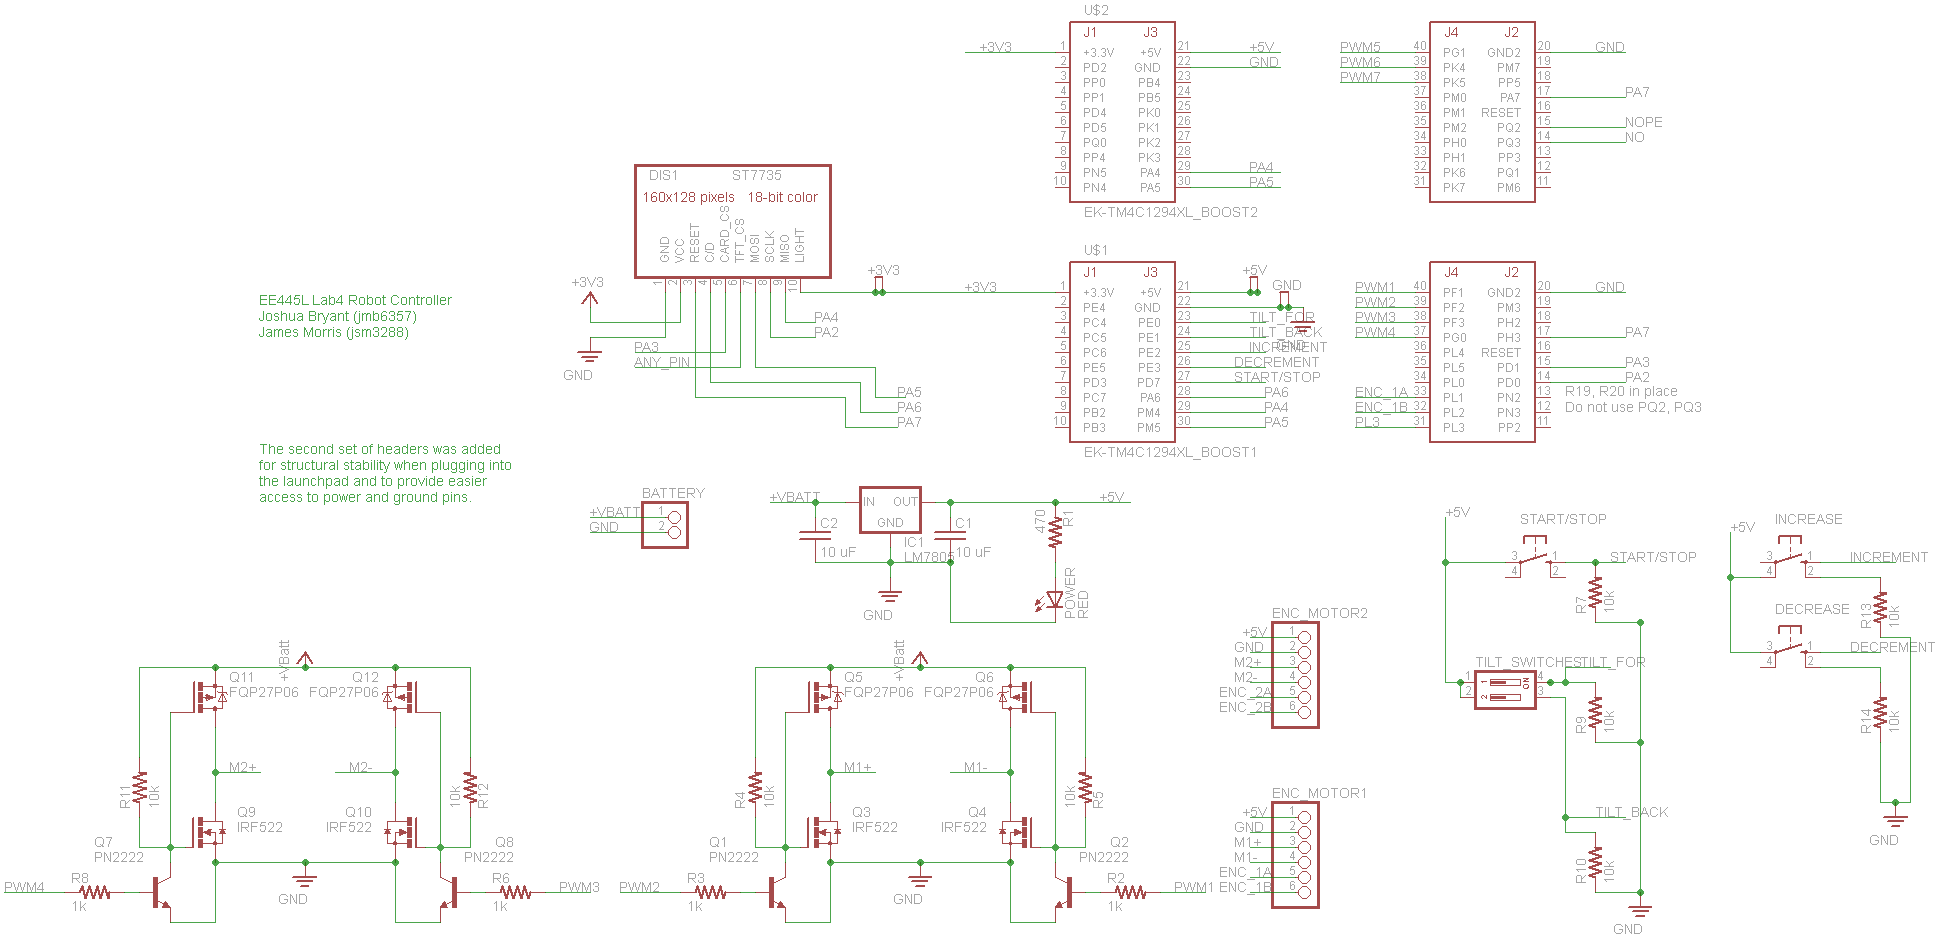
\includegraphics[keepaspectratio, angle = 90, width=0.5\textwidth]{Lab7Graphics/Schematic.png}
		\caption{Schematic for Generic Robot Controller}
		\label{fig:schematic}
	\end{figure}
	
	\begin{figure}[h]
		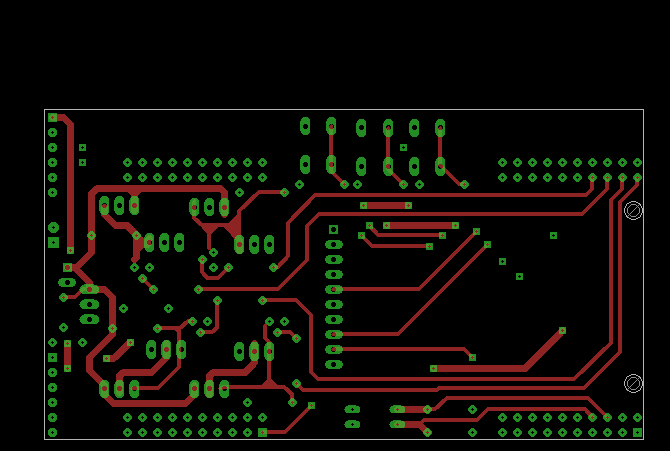
\includegraphics[keepaspectratio, width = \textwidth]{Lab7Graphics/PCB_Top}
		\caption{PCB Layout: Top Layer}
		\label{fig:PCB_Top}
	\end{figure}
	
	\begin{figure}[h]
		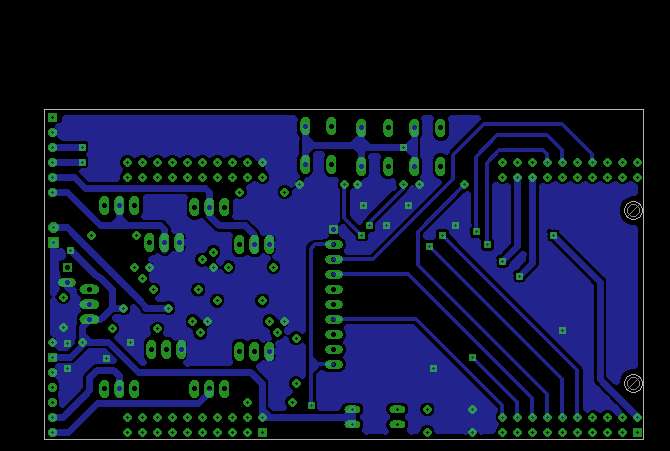
\includegraphics[keepaspectratio, width = \textwidth]{Lab7Graphics/PCB_Bottom}
		\caption{PCB Layout: Bottom Layer}
		\label{fig:PCB_Bottom}
	\end{figure}
	
	\begin{figure}[h]
		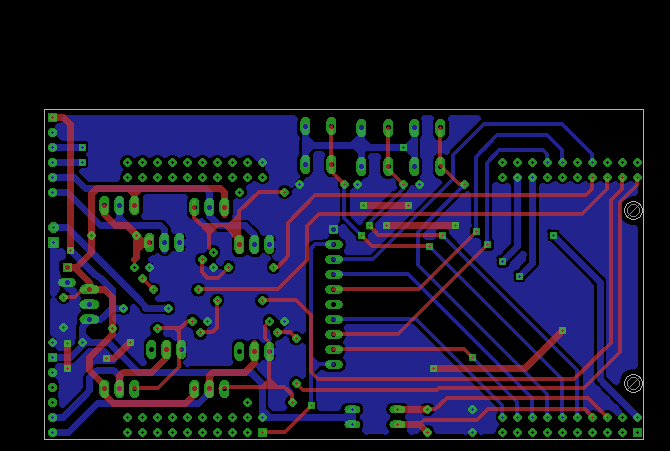
\includegraphics[keepaspectratio, width = \textwidth]{lab7Graphics/PCB_Combined}
		\caption{PCB Layout: Tob and Bottom Layers Combined}
		\label{fig:PCB_Combined}
	\end{figure}
	

%----------------------------------------------------------------------------------------
%	SECTION 3 Software Design
%----------------------------------------------------------------------------------------

%----------------------------------------------------------------------------------------
%	SECTION 4 Measurement Data
%----------------------------------------------------------------------------------------
\section{Measurement Data}
	\subsection{Estimated Current}
		In Lab 4 we measured the current of the system with the motor running at full speed was 209 mA while the current of the motor itself spinning was 105 mA. This gives an approximate current for the system in Lab 4 sans motor being $\sim$110 mA. The circuit for this lab is very similar to that of Lab 4 with the addition of two full H-bridges meaning the current of the system at rest without any motor can be estimated as the sum of the current from Lab 4 and the zero gate voltage drain current. This comes out to $110 mA + 8*(250 \mu A) = 112 mA$. So at rest, the system is estimated to consume 110$\sim$115 mA. With the addition of motors, the current through the system will increase dramatically and be driven mostly by the motors. For the final project demonstration, we are currently planning on using up to 1 motor that will likely use about 2 A leading to a total system current of $\sim$ 2.15 A at peak. This is fine since the peak current output of the voltage regulator on board the booster pack can output up to 2.4 A continuously at room temperature.
	
	\subsection{Estimated Cost}
		The estimated cost of the booster pack is $\sim$\$27.00. This is not including the TM4C1294 board in the price. 

%----------------------------------------------------------------------------------------
%	SECTION 5 Analysis and Discussion
%----------------------------------------------------------------------------------------



\end{document}